\chapter{\IfLanguageName{dutch}{Architectuurprincipes en prestatieanalyse}{Architecture principles and performance analysis}}
\label{ch:testen-prestatieanalyse}

\section{Inleiding}

In dit hoofdstuk worden de principes van de applicatiearchitectuur en de prestatieanalyse besproken. Voor de load testing van de applicatie wordt gebruikgemaakt van \textit{ReadyAPI}, een tool die ons in staat stelt de prestaties van de applicatie te testen door het simuleren van een groot aantal gebruikers die tegelijkertijd toegang proberen te krijgen tot de applicatie.

\section{Architectuurprincipes}

\subsection{Discoverability}

Discoverability verwijst naar het gemak waarmee de verschillende services en hun functionaliteiten kunnen worden gevonden en gebruikt binnen een microservices-architectuur. Dit aspect is cruciaal voor de efficiëntie en het onderhoud van de applicatie, aangezien het helpt bij het snel identificeren van de juiste services voor specifieke taken.

Er zijn 2 aspecten van discoverability die belangrijk zijn bij het ontwerpen van een microservices architectuur. Het technische aspect verwijst naar het vermogen van services om elkaar te vinden en met elkaar te communiceren binnen een netwerk. Het operationele aspect verwijst naar het vermogen van ontwikkelaars en beheerders om de services te vinden en te begrijpen.

Om een call te doen naar een andere service moet enkel de naam van de service en de poort waarop deze draait gekend zijn. Dit is mogelijk door de service discovery van Istio. Hierdoor kunnen services elkaar vinden en met elkaar communiceren zonder dat de locatie van de service gekend moet zijn.

Voor het operationele aspect bieden de meeste servicemeshes een dashboard aan waarin de services en hun interacties visueel worden weergegeven. Dit maakt het gemakkelijk voor ontwikkelaars en beheerders om de services te vinden en te begrijpen. In Istio is dit het Kiali-dashboard \ref{fig:kaili} \ref{fig:kialiServices}.

\begin{figure}[H]
    \centering	
    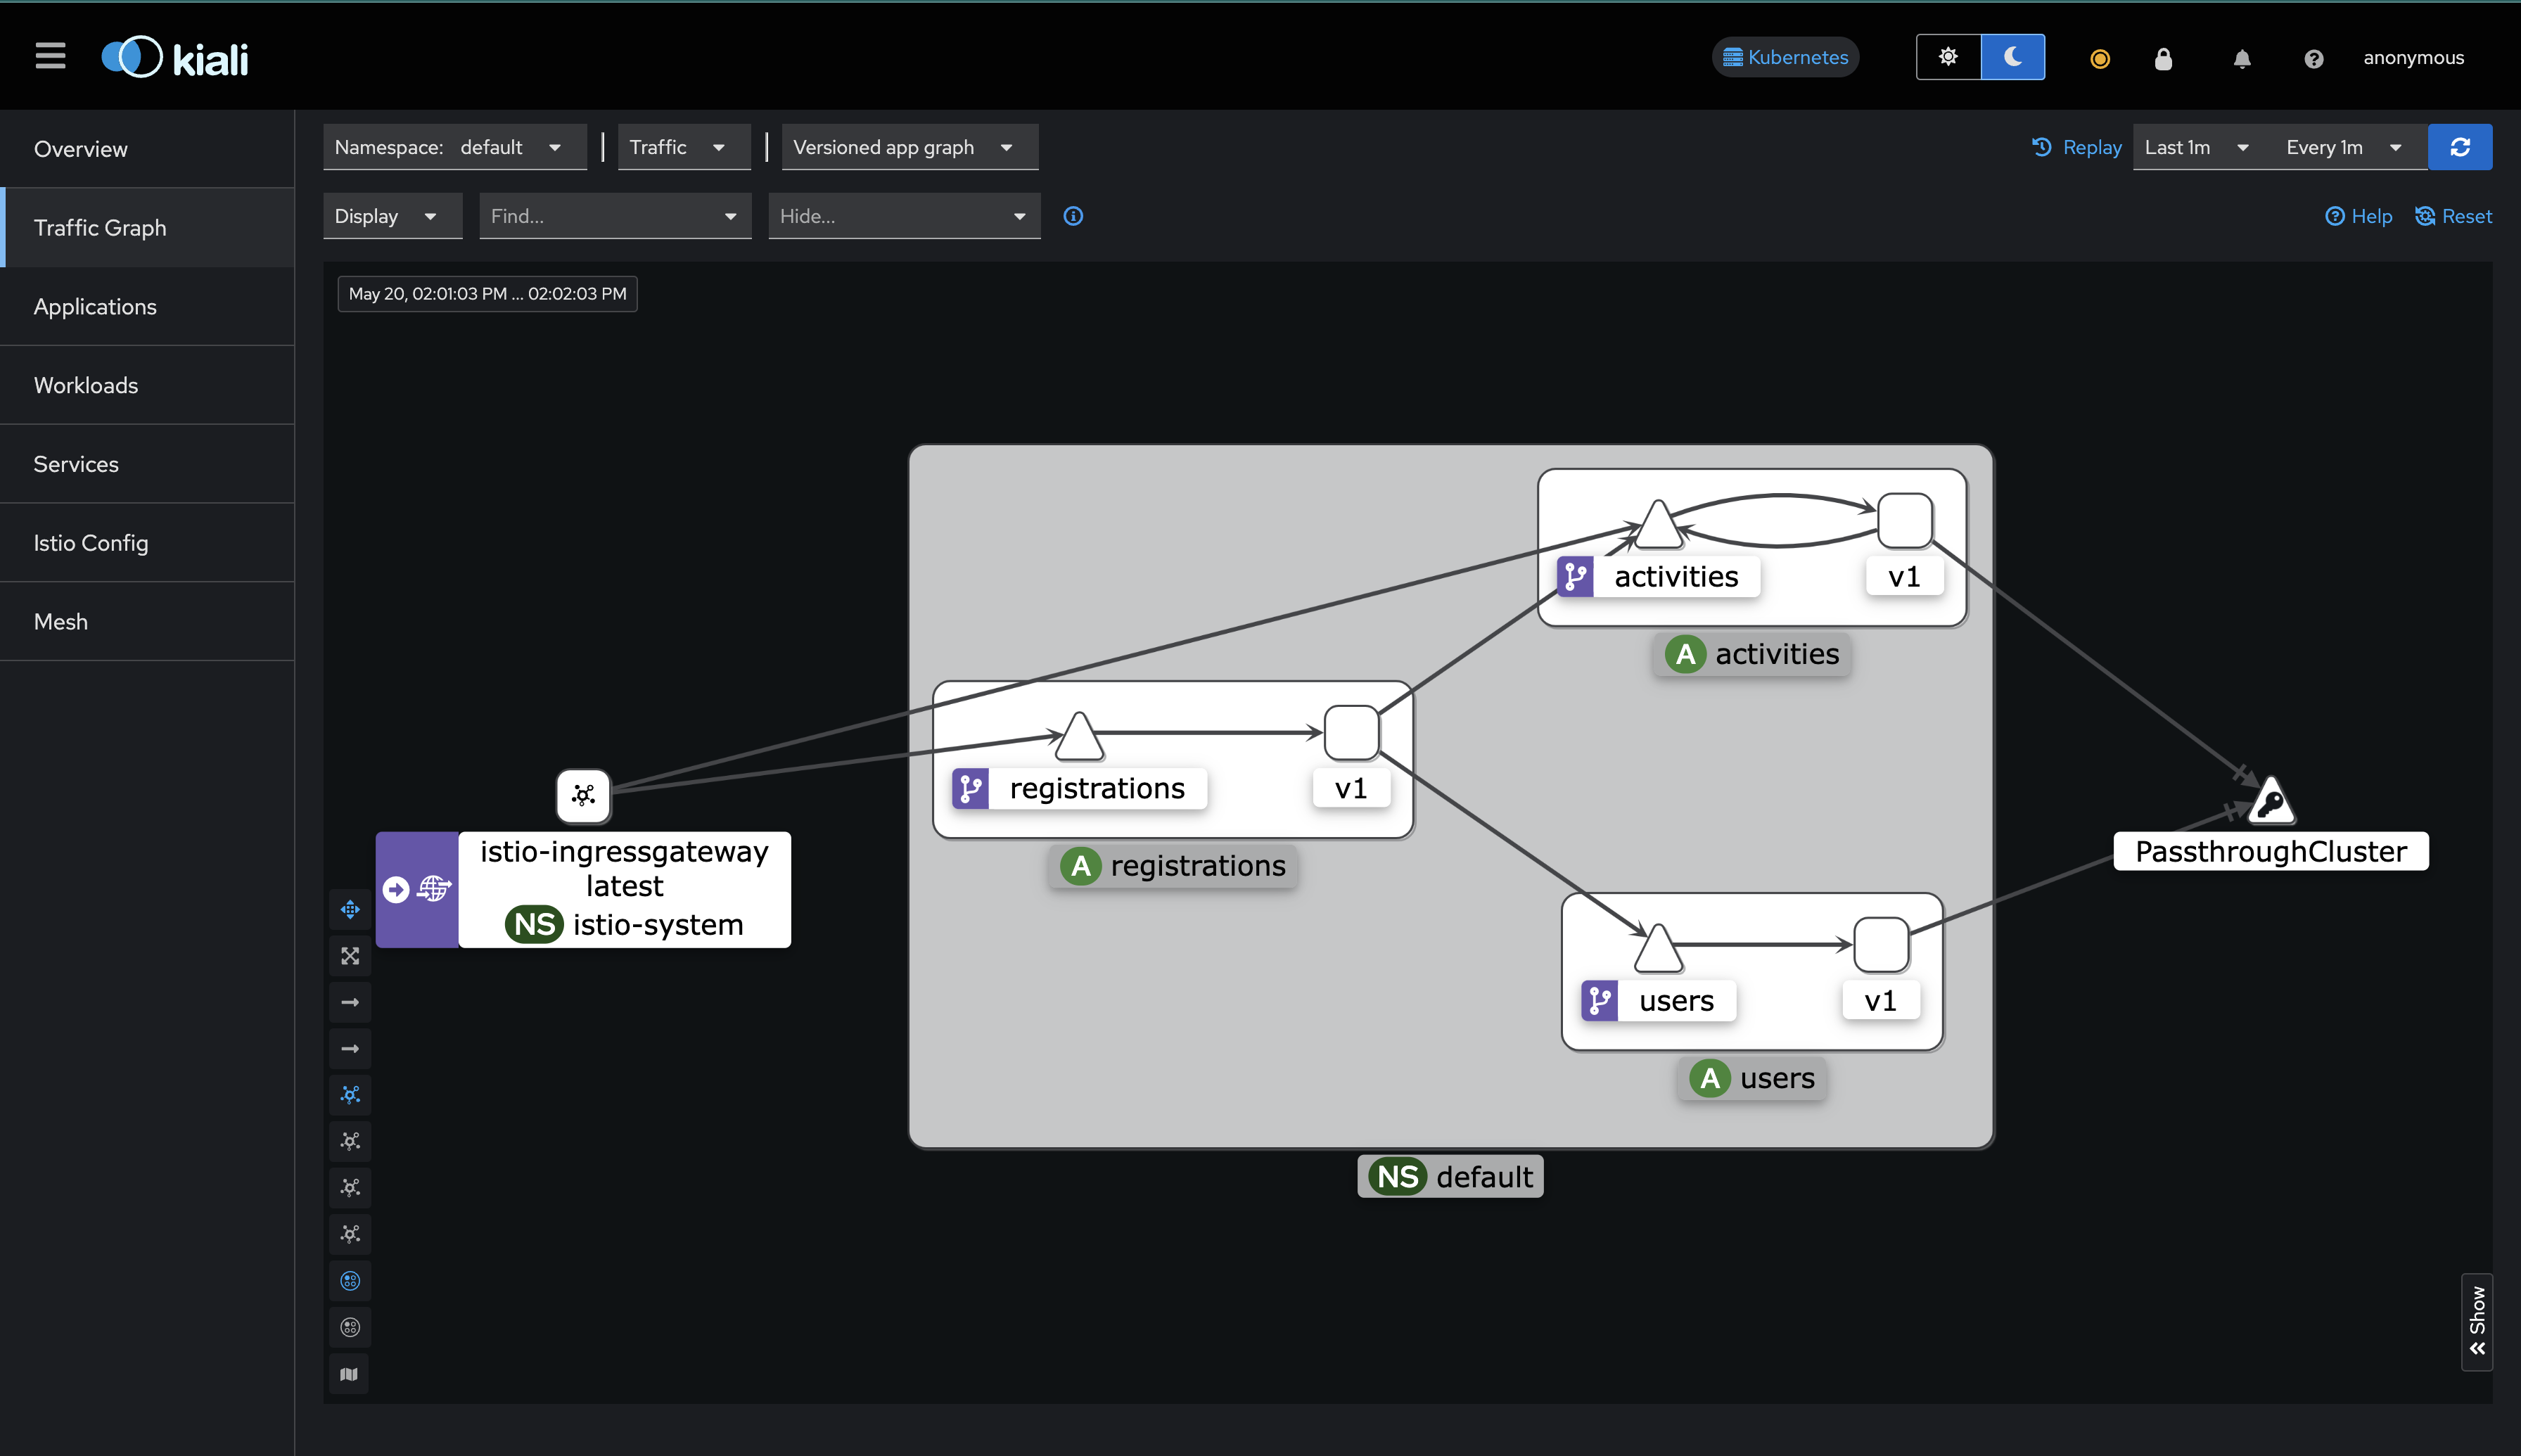
\includegraphics[width = 16cm]{kiali.png} 
    \caption{Kiali Console} 
    \label{fig:kaili}
\end{figure}

\begin{figure}[H]
    \centering	
    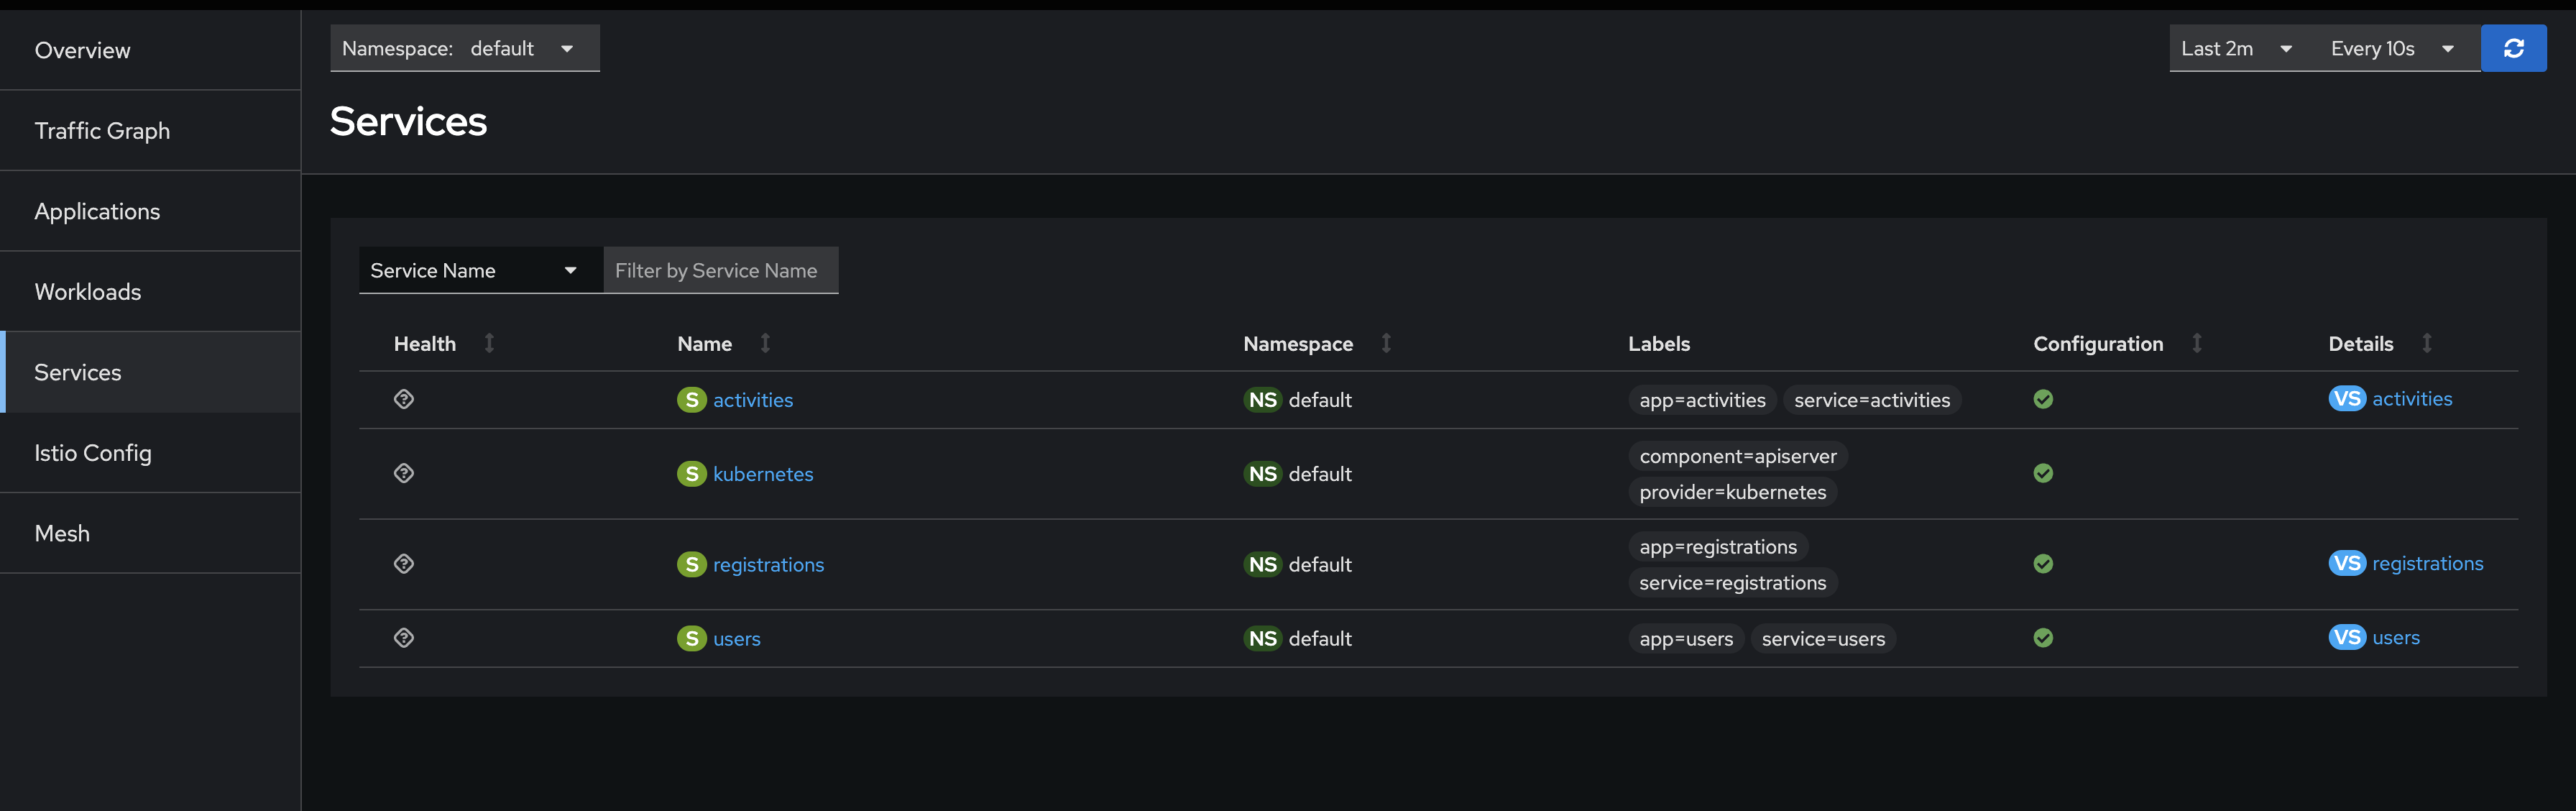
\includegraphics[width = 16cm]{kialiServices.png} 
    \caption{Kiali Console met services} 
    \label{fig:kialiServices}
\end{figure}


\subsection{Schaalbaarheid}

Schaalbaarheid is een belangrijke eigenschap van microservices, omdat ze onafhankelijk van elkaar kunnen worden geschaald. Dit betekent dat we de resources van elke service afzonderlijk kunnen verhogen om de prestaties van de applicatie te verbeteren. Door het aantal replica's van een service te verhogen, kunnen we de belasting verdelen over meerdere instanties en zo de prestaties van de applicatie verbeteren.

Om de schaalbaarheid te testen, hebben we simulaties uitgevoerd met verschillende aantallen replica's: 1, 2 en 10. De resultaten van deze tests zijn weergegeven in de figuren \ref{fig:1replica}, \ref{fig:2replica}   en \ref{fig:10replica}.

\begin{figure}[H]
    \centering	
    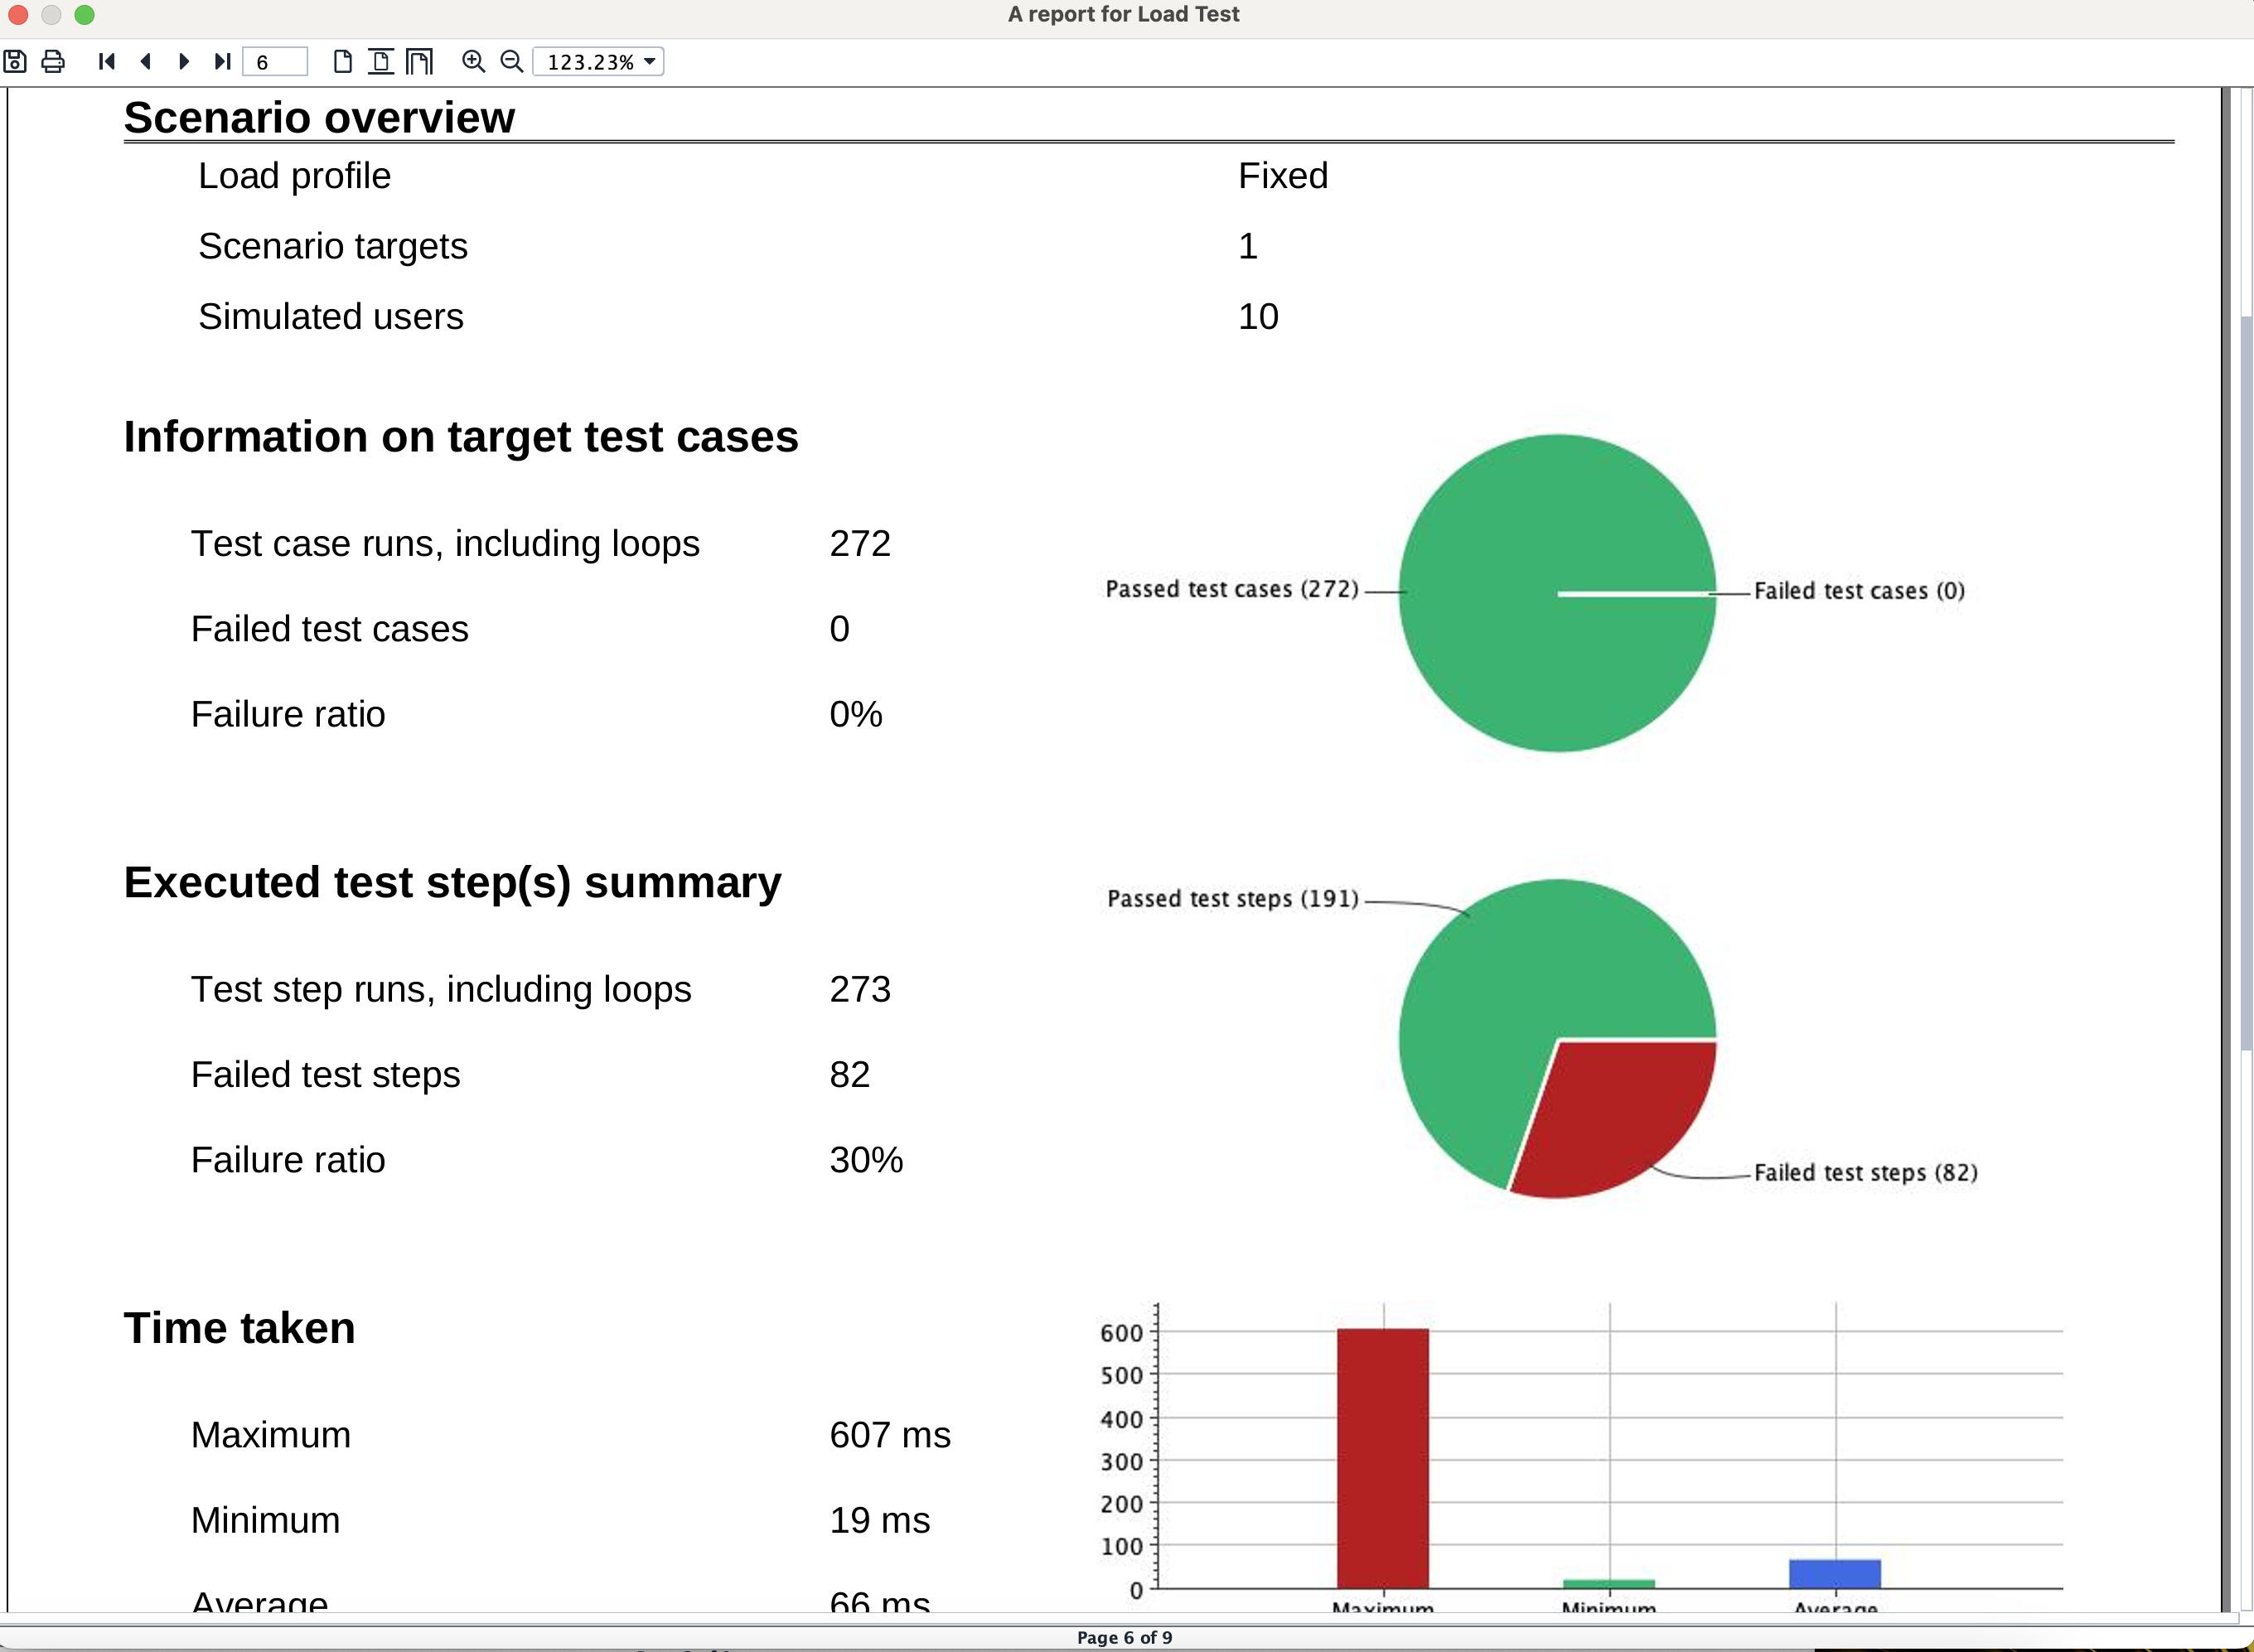
\includegraphics[width=12cm]{10sim1rep.png}
    \caption{10 simulaties op 1 replica} 
    \label{fig:1replica}
\end{figure}

\begin{figure}[H]
    \centering	
    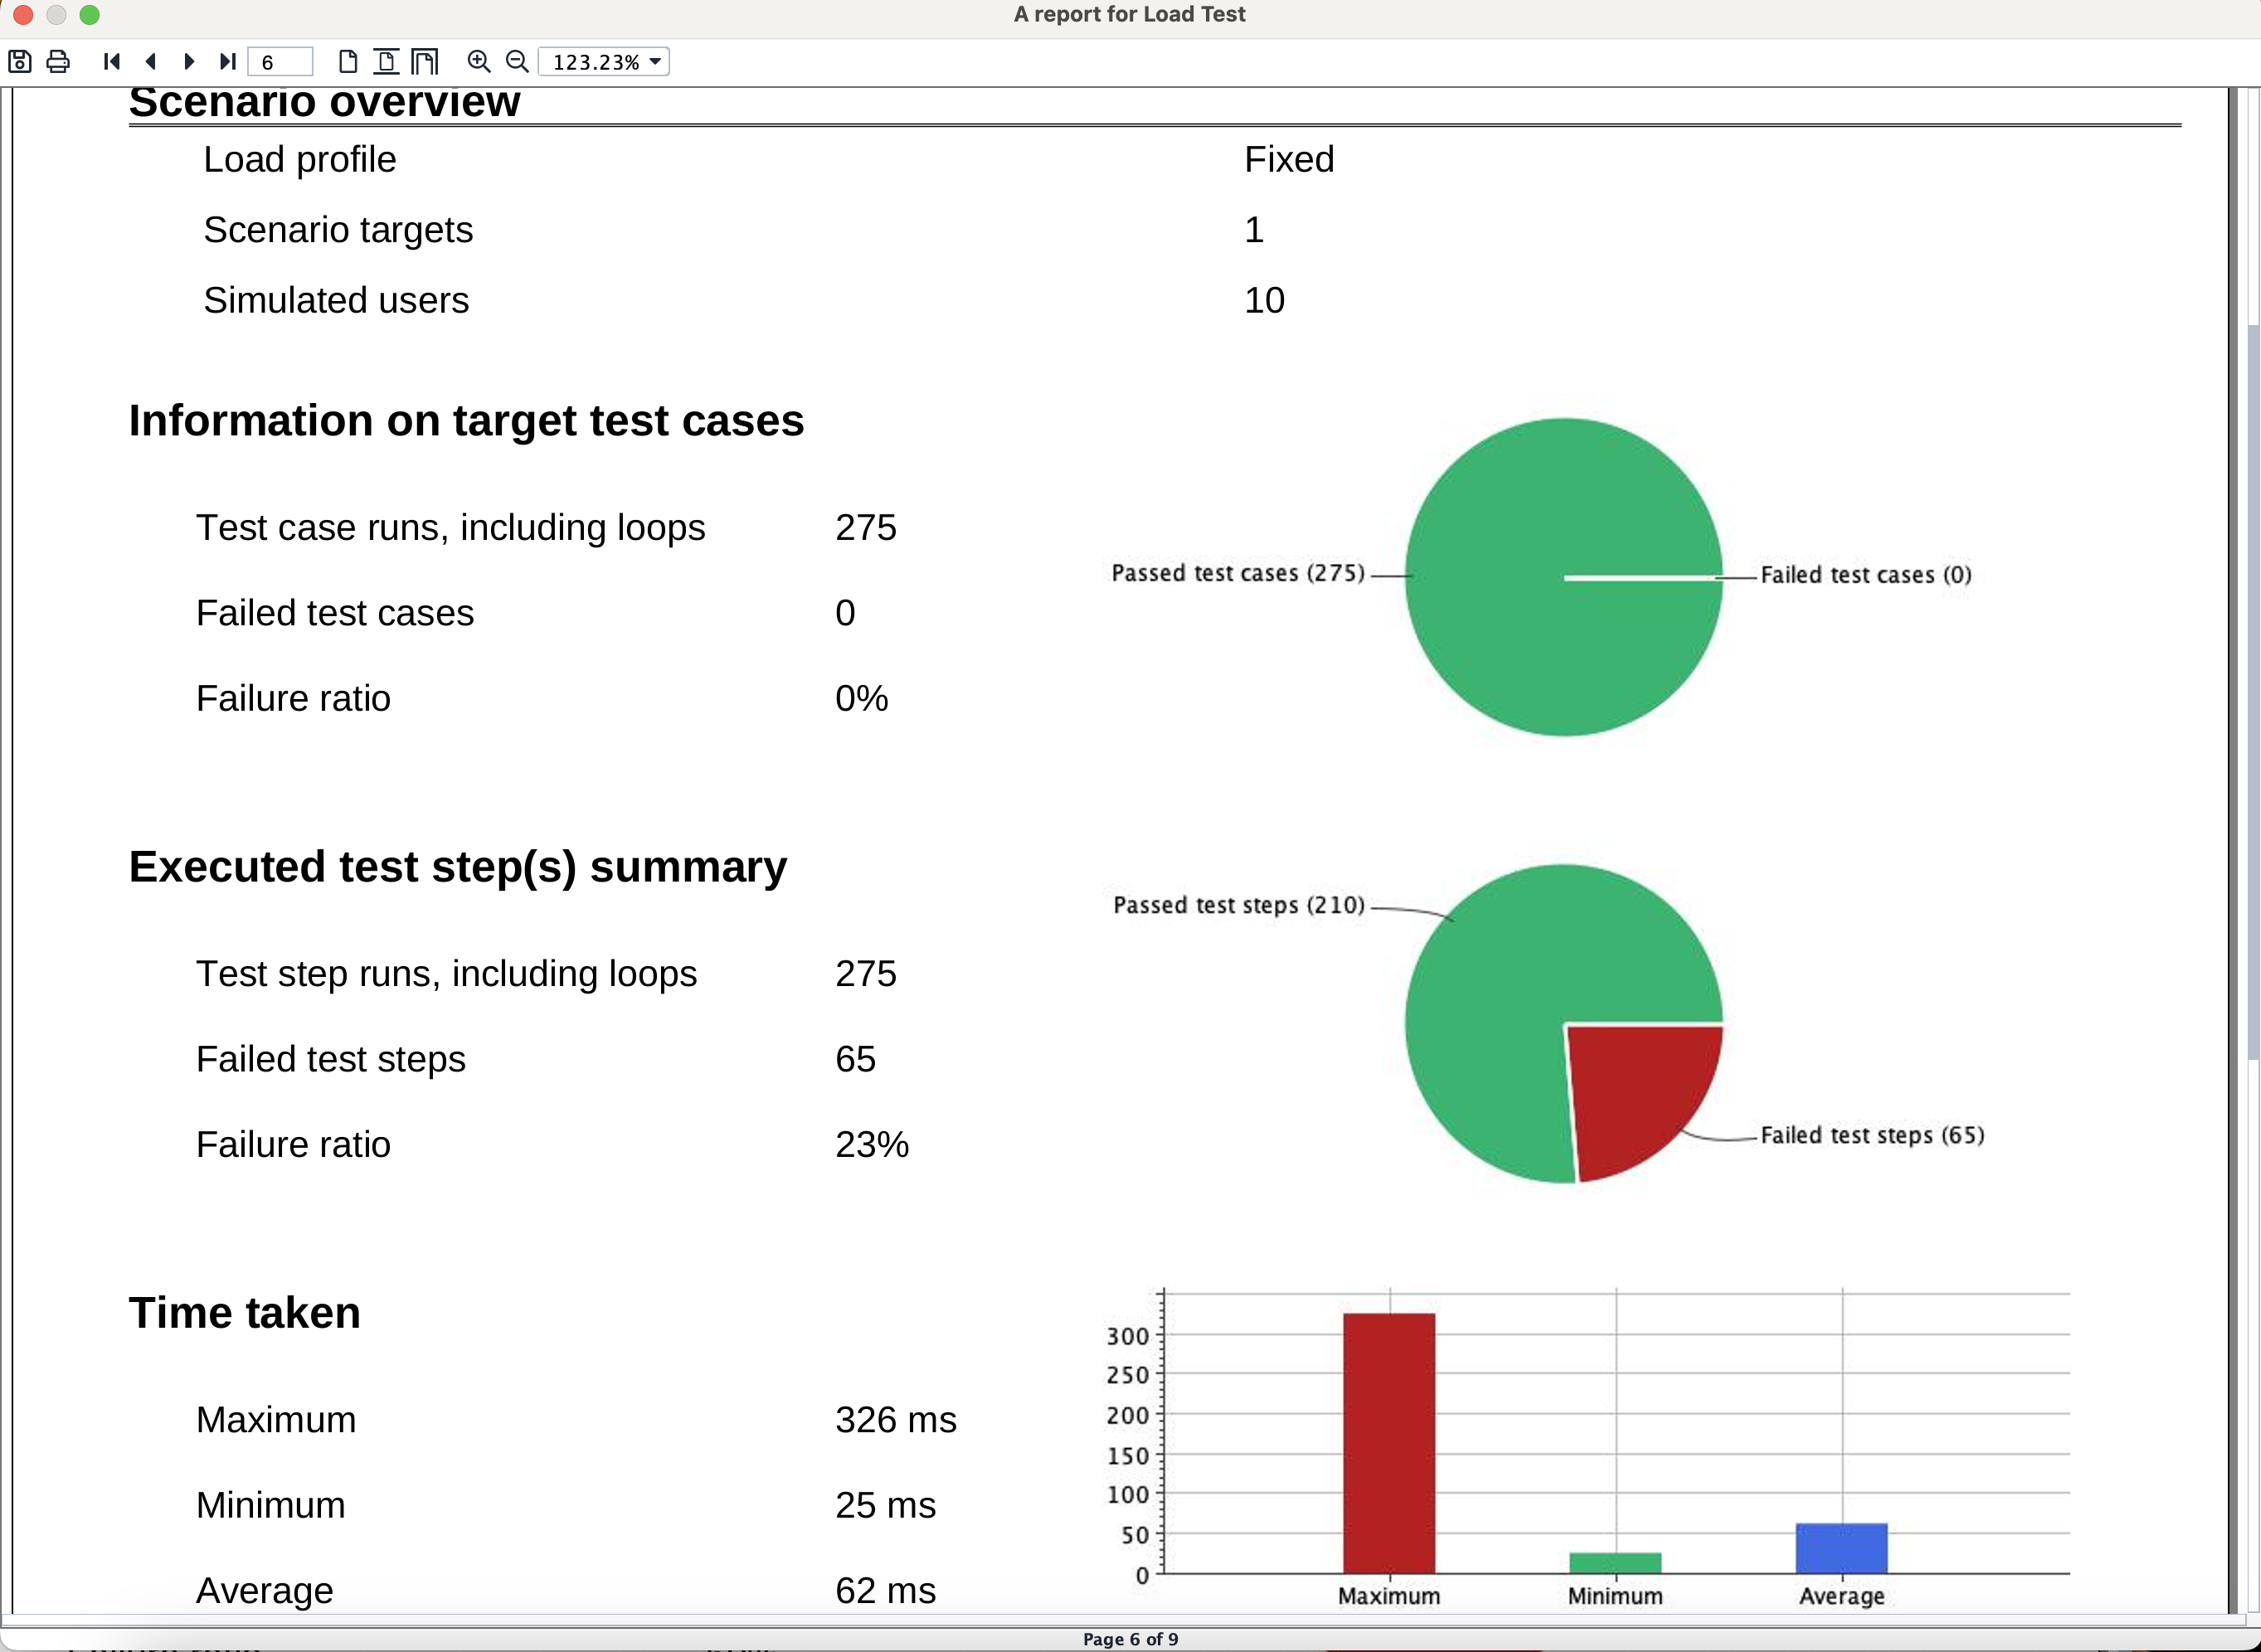
\includegraphics[width=12cm]{10sim2rep.png}
    \caption{10 simulaties op 2 replica's} 
    \label{fig:2replica}
\end{figure}

\begin{figure}[H]
    \centering	
    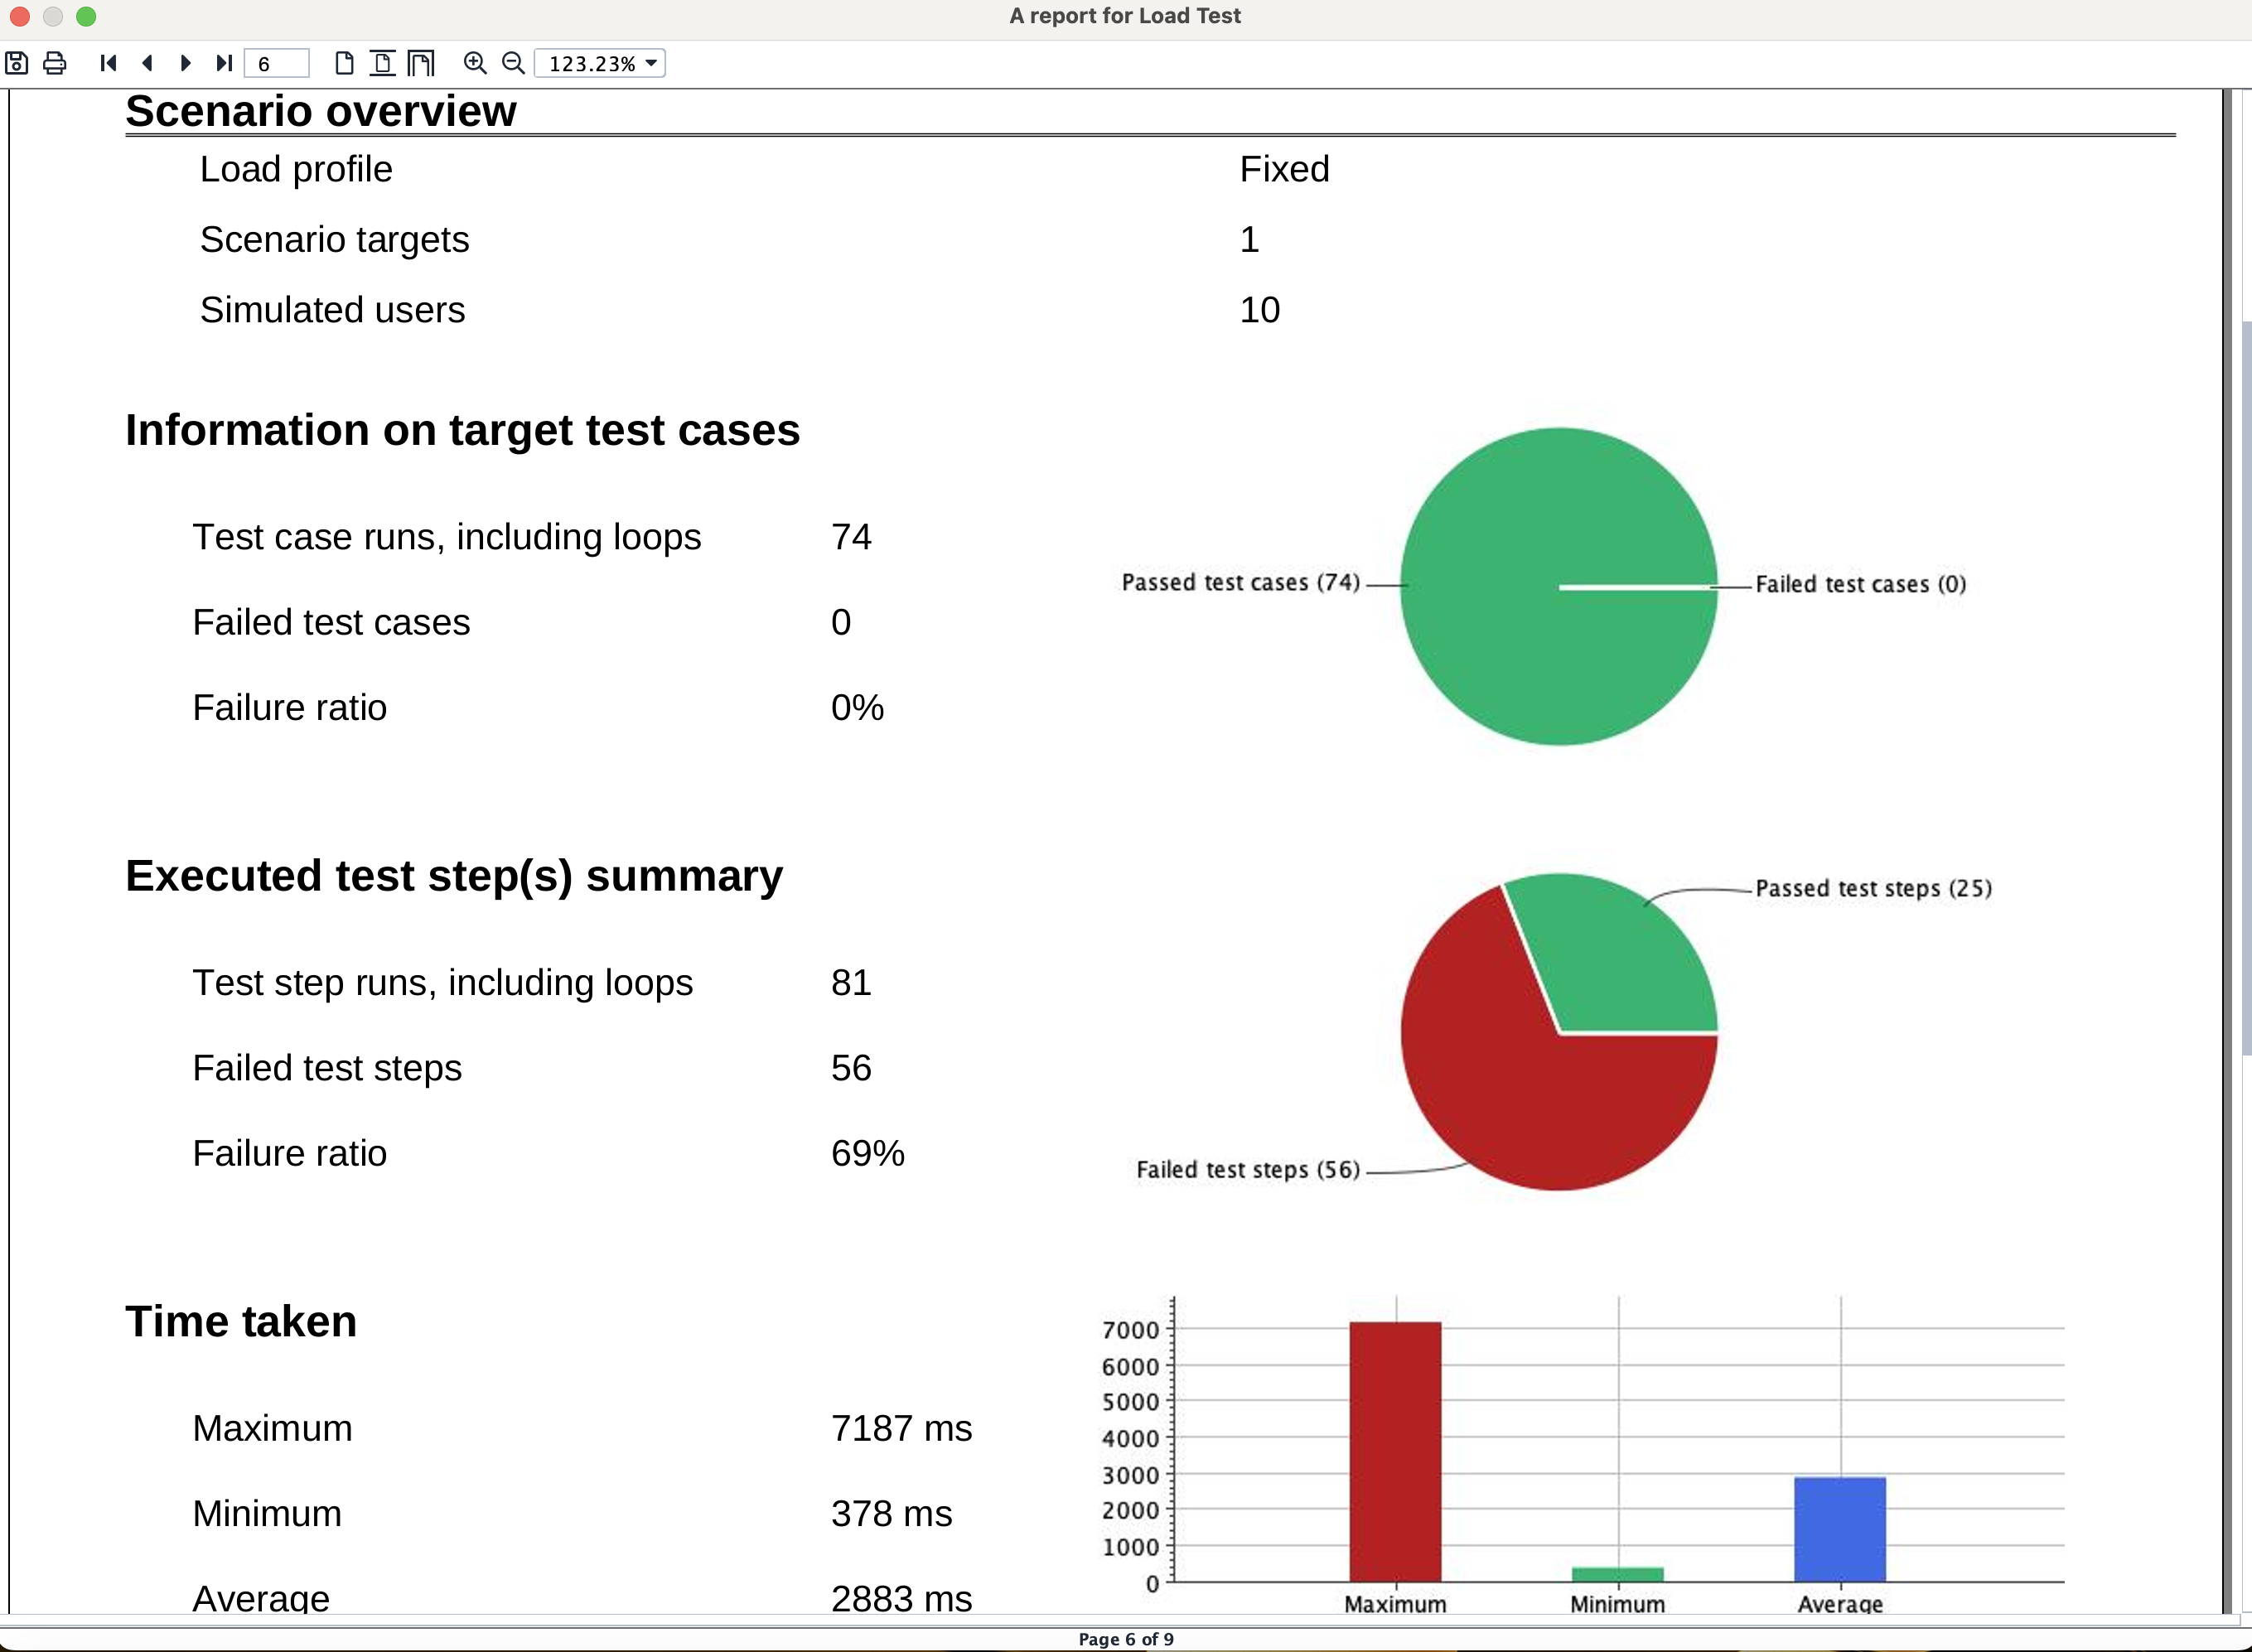
\includegraphics[width=12cm]{10sim10rep.png}
    \caption{10 simulaties op 10 replica's} 
    \label{fig:10replica}
\end{figure}

Uit de resultaten blijkt dat bij het verhogen van het aantal replica's de prestaties verbeteren tot een bepaald punt. Bij 2 replica's zijn de testsuccespercentages hoger en zijn er minder time-outs. 

Bij het draaien van 10 replica's zijn de recources van mijn desktop overbelast. Er is wel te zien dat bij het opschalen van de replica's de prestaties verbeteren tot het punt waarop de infrastructuur overbelast raakt.

Dit komt omdat mijn infrastructuur (desktop) niet mee kan schalen met het aantal replica's wat in een professionele omgeving wel zou kunnen.

Theoretisch zijn microservices oneindig horizontaal schaalbaar, terwijl monolieten meestal enkel verticaal schaalbaar zijn. Dit beperkt de schaalbaarheid van monolieten tot de maximale grootte van de servers waarop ze draaien.

Verticaal schalen is meer kracht aan de server toevoegen, terwijl horizontaal schalen het toevoegen van meer servers is.


\section{Prestatieanalyse}

\subsection{Responstijd}

De responstijd is een kritieke prestatie-indicator voor de applicatie. Voor het testen van de responstijd hebben we gebruikgemaakt van \textit{ReadyAPI} om zowel een monolithische versie van de applicatie als de microservices-versie te testen. De resultaten zijn weergegeven in de figuren \ref{fig:monolietTimeTest} en \ref{fig:microservicesTimeTest}.

\subsubsection*{Health check - single threaded}

Als eerste test wordt een single threaded health check uitgevoerd op beide systemen. Hiermee wordt gekeken wat de impact is van de architectuur op de responstijd van de applicatie. De resultaten van deze test zijn weergegeven in de figuren \ref{fig:monolietTimeHealth} en \ref{fig:microservicesTimeHealth}.

\begin{figure}[H]
    \centering	
    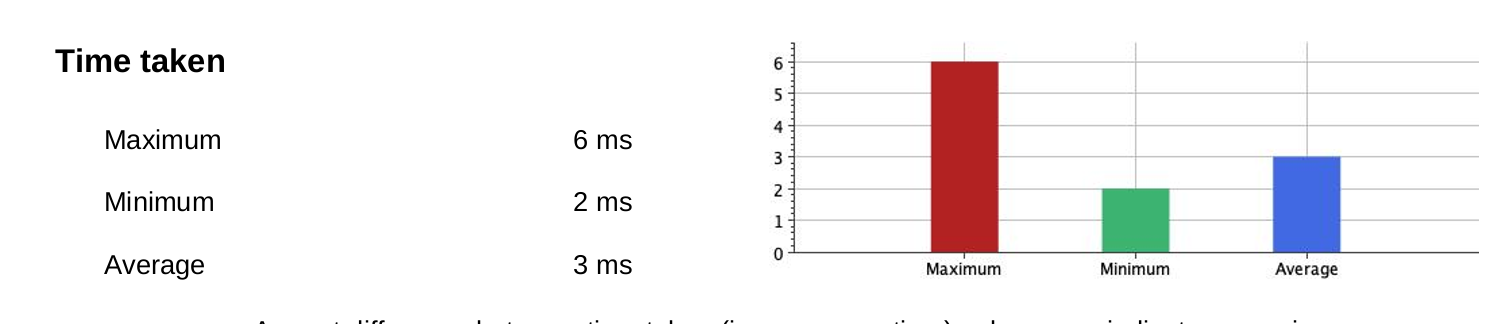
\includegraphics[width=12cm]{monolietTimeHealth.png}
    \caption{Responstijd monoliet health check} 
    \label{fig:monolietTimeHealth}
\end{figure}

\begin{figure}[H]
    \centering	
    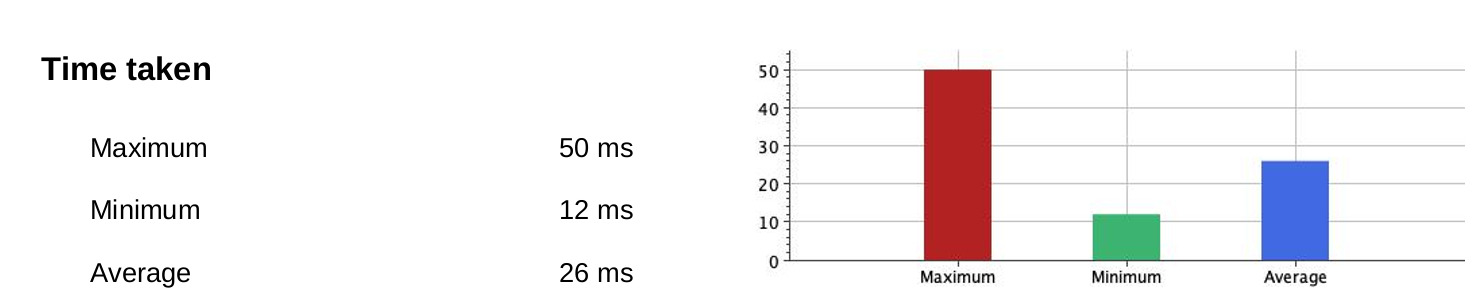
\includegraphics[width=12cm]{microservicesTimeHealth.png}
    \caption{Responstijd microservices health check} 
    \label{fig:microservicesTimeHealth}
\end{figure}

Uit de resultaten blijkt dat de responstijd van de monoliet lager is dan die van de microservices. Bij de monoliet applicatie wordt rechtstreeks een HTTP call gedaan naar de API, terwijl bij de microservices de API calls worden gedaan via een ingressgateway, sidecar proxy en dan pas naar de API. Dit verklaart waarschijnlijk waarom de responstijd van de microservices hoger is dan die van de monoliet.
\subsubsection*{Health check - multi threaded}
Als volgende test wordt een multi-threaded health check uitgevoerd op beide systemen. Hiermee wordt gekeken wat de impact is van de architectuur op de responstijd van de applicatie. De resultaten van deze test zijn weergegeven in de figuren \ref{fig:monolietTimeHealthMulti} en \ref{fig:microservicesTimeHealthMulti}.

\begin{figure}[H]
    \centering	
    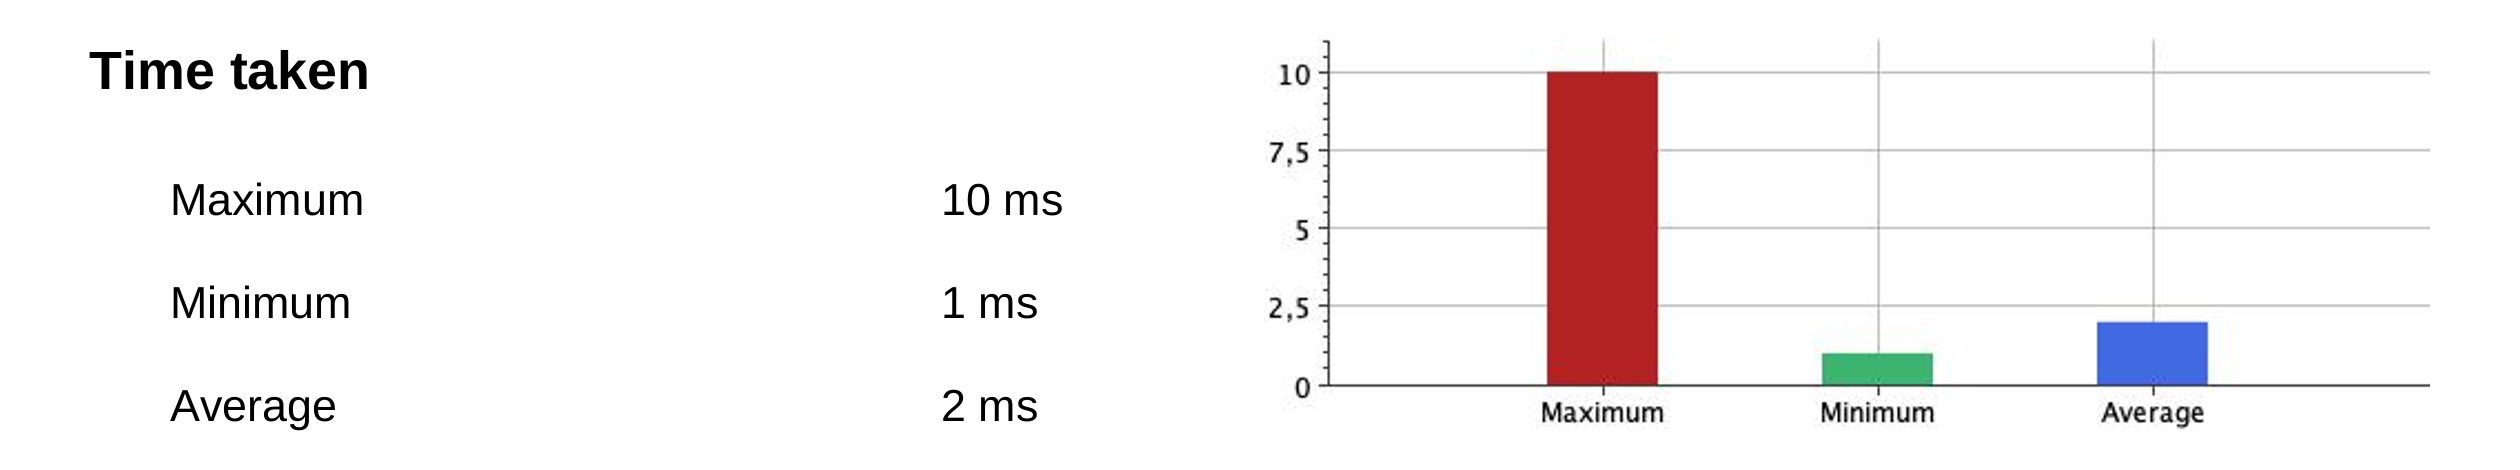
\includegraphics[width=12cm]{monolietTimeHealthMulti.png}
    \caption{Responstijd monoliet health check multi-threaded} 
    \label{fig:monolietTimeHealthMulti}
\end{figure}

\begin{figure}[H]
    \centering	
    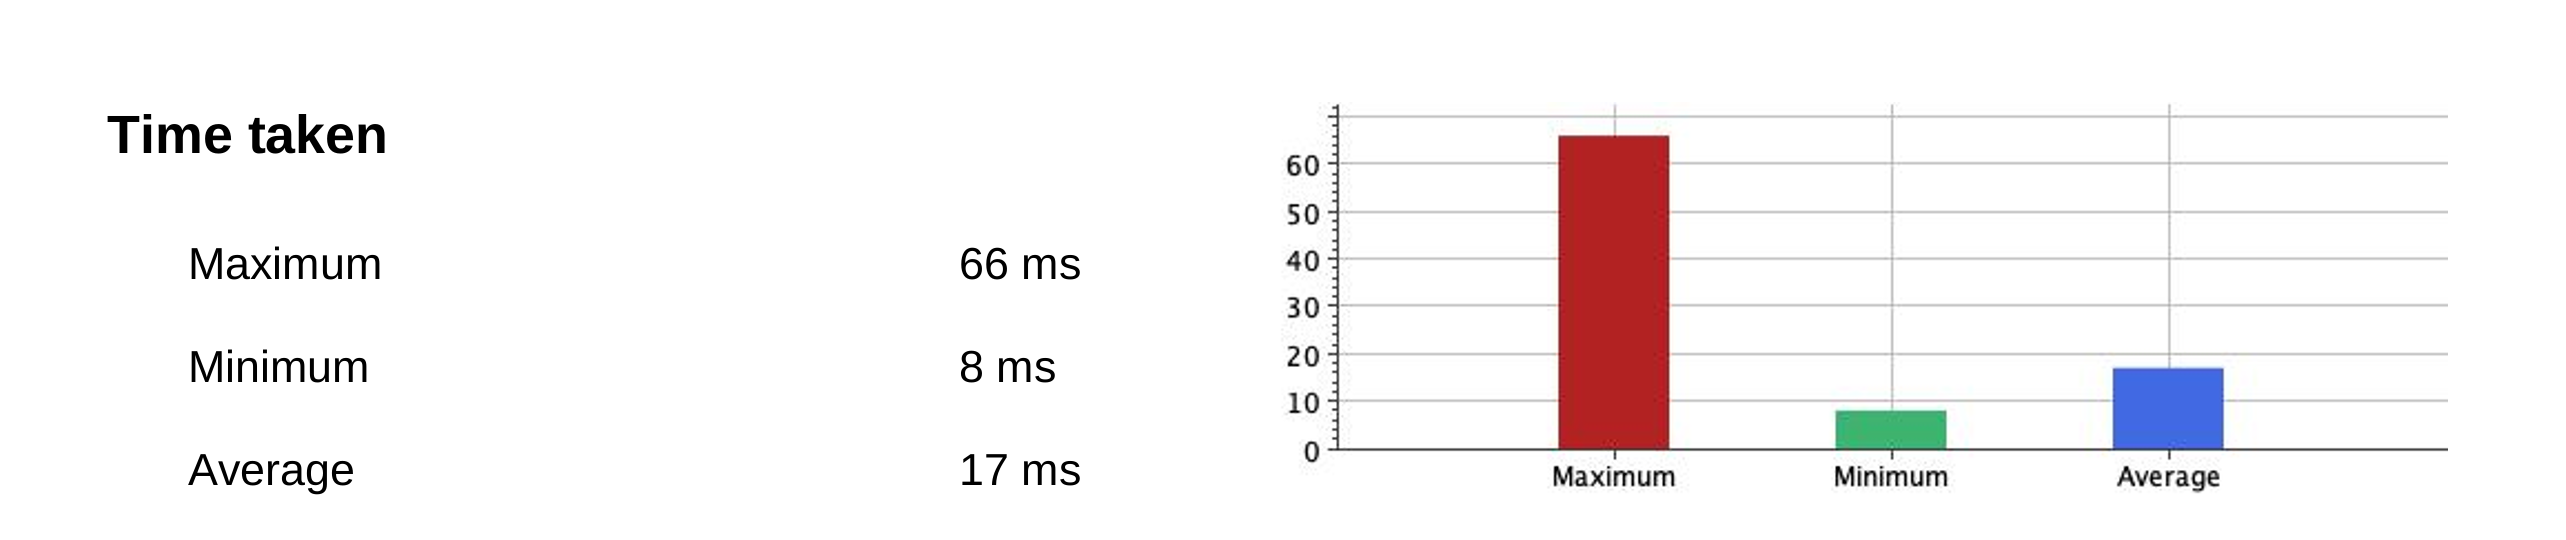
\includegraphics[width=12cm]{microservicesTimeHealthMulti.png}
    \caption{Responstijd microservices health check multi-threaded} 
    \label{fig:microservicesTimeHealthMulti}
\end{figure}

Er is dus geen significant verschil in responstijd bij een multi-threaded health check ten opzichte van single threaded. Het lijkt dus dat beide architecturen hetzelfde aantal requests aankunnen.
\subsubsection*{Service to service invocation}
Als laatste test wordt een api aangeroepen die de registraties voor een activiteit ophaalt samen met de details van de activiteit. Hiermee wordt gekeken wat de impact is van de architectuur op de responstijd van de applicatie. De resultaten van deze test zijn weergegeven in de figuren \ref{fig:monolietTimeTest} en \ref{fig:microservicesTimeTest}.

In de monoliet wordt dit gedaan door een join in de repository laag, terwijl in de microservice de registratieservice de activiteitenservice aanroept.

\begin{figure}[H]
    \centering	
    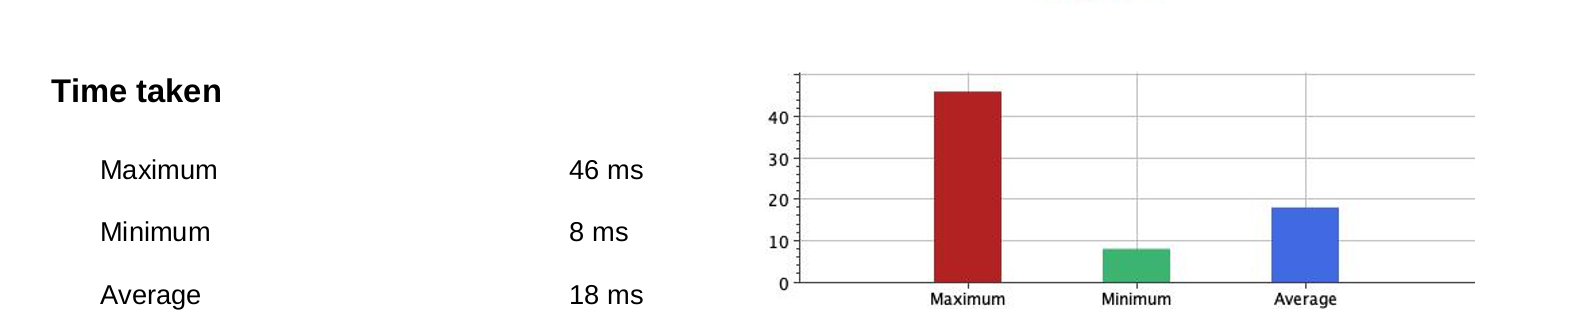
\includegraphics[width=12cm]{monolietTimeTest.png}
    \caption{Responstijd monoliet} 
    \label{fig:monolietTimeTest}
\end{figure}

\begin{figure}[H]
    \centering	
    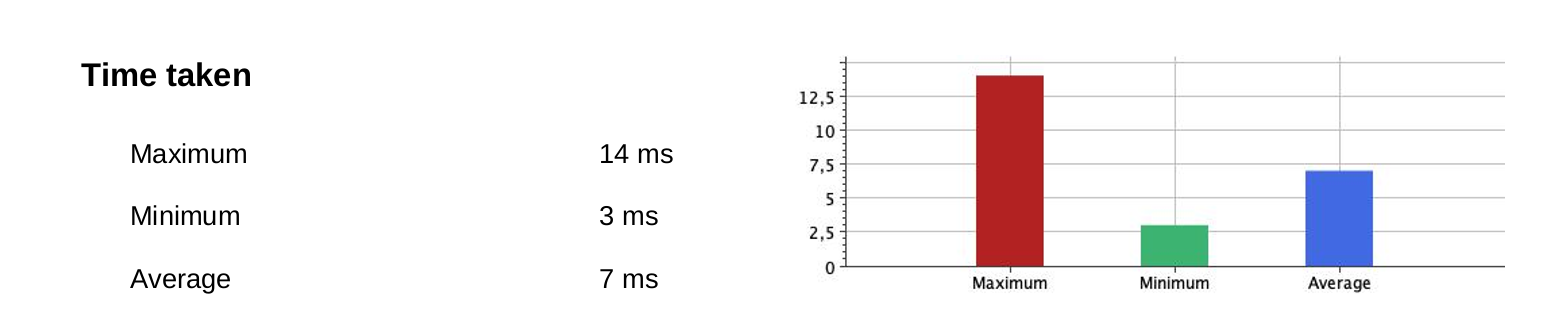
\includegraphics[width=12cm]{microservicesTimeTest.png}
    \caption{Responstijd microservices} 
    \label{fig:microservicesTimeTest}
\end{figure}

Er is geen significant verschil tussen de responstijden in deze testen en de voorafgaande testen. Het lijkt dus dat de service to service calls minder impact hebben op de response tijd dan de ingress calls. Om deze calls zoveel mogelijk te beperken zou de UI zelf of een facade service voor de UI binnen de servicemesh kunnen gedraaid worden.


De responstijd van de monoliet is lager omdat alle functionaliteiten zich binnen één enkele backend bevinden, waardoor de communicatie tussen de verschillende delen van de applicatie efficiënter verloopt.

\subsection{Robuustheid}

Robuustheid betreft het vermogen van de applicatie om correct te blijven functioneren onder uiteenlopende omstandigheden, zoals hoge belasting of onverwachte gebeurtenissen.

Zowel de monoliet als de microservices hebben één of meerdere single points of failure. Bij een monoliet is dit de applicatie zelf, terwijl dit bij onze microservices de ingressgateway is. Het is dus belangrijk om deze single points of failure te identificeren en hen zo robust mogelijk te maken.
Dit is een uitdaging die voor beide architecturen geldt.

Bij microservices worden de risico's verspreid omdat elke service zijn eigen infrastructuur heeft. Het falen van een van deze componenten heeft een beperkte impact op de volledige functionaliteit van de applicatie. Bij monolithische architecturen kan de volledige functionaliteit snel in gevaar komen.
